\documentclass[border=4pt]{standalone}
% Shared typography and colours for the standalone figures.
\usepackage{unicode-math}
\setmainfont{TeX Gyre Heros}
\setmathfont{TeX Gyre Pagella Math}
\usepackage{tikz}
\usetikzlibrary{arrows.meta,positioning,calc,decorations.pathreplacing}
\usepackage{pgfplots}
\pgfplotsset{compat=1.18}

% One colour per element or subsystem. Record the mapping in
% the working repository conventions and use it identically in every figure.
\definecolor{elemA}{HTML}{1F5FA8}
\definecolor{elemB}{HTML}{B8461B}
\definecolor{elemC}{HTML}{2E7D32}
\definecolor{elemD}{HTML}{6A4C93}
\definecolor{frameline}{HTML}{555555}

\begin{document}
\hyphenpenalty=10000
\exhyphenpenalty=10000
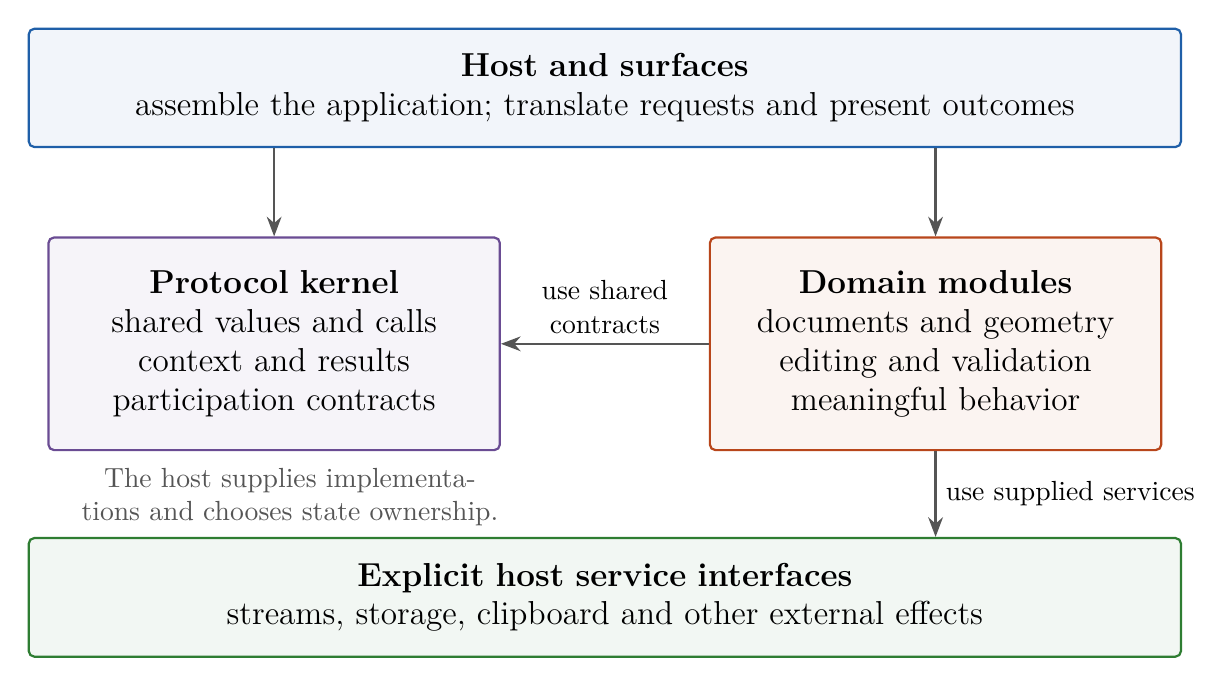
\begin{tikzpicture}[
  box/.style={draw,rounded corners=2pt,thick,align=center,inner sep=9pt,font=\large},
  arrow/.style={-{Stealth[length=2.5mm]},thick,draw=frameline}
]
\node[box,draw=elemA,fill=elemA!6,text width=14cm] (host) at (0,3.25)
  {\textbf{Host and surfaces}\\assemble the application; translate requests and present outcomes};
\node[box,draw=elemD,fill=elemD!6,text width=5.1cm,minimum height=2.7cm] (kernel) at (-4.2,0)
  {\textbf{Protocol kernel}\\shared values and calls\\context and results\\participation contracts};
\node[box,draw=elemB,fill=elemB!6,text width=5.1cm,minimum height=2.7cm] (domain) at (4.2,0)
  {\textbf{Domain modules}\\documents and geometry\\editing and validation\\meaningful behavior};
\draw[arrow] (host.south -| kernel.north) -- (kernel.north);
\draw[arrow] (host.south -| domain.north) -- (domain.north);
\draw[arrow] (domain.west) -- node[above,align=center,font=\normalsize] {use shared\\contracts} (kernel.east);
\node[box,draw=elemC,fill=elemC!6,text width=14cm] (services) at (0,-3.22)
  {\textbf{Explicit host service interfaces}\\streams, storage, clipboard and other external effects};
\draw[arrow] (domain.south) -- node[right,font=\normalsize] {use supplied services} (services.north -| domain.south);
\node[align=center,text=frameline,font=\normalsize,text width=6cm] at (-4,-1.95)
  {The host supplies implementations and chooses state ownership.};
\end{tikzpicture}
\end{document}
